\documentclass{article}
\usepackage[T1]{fontenc}
\usepackage[utf8]{inputenc}
\usepackage[margin=1in]{geometry}
\usepackage{fancyhdr} 
\usepackage{listings}
\usepackage[ruled,vlined]{algorithm2e}
\usepackage{amsthm}
\usepackage{amsfonts}
\usepackage{amssymb}
\usepackage{graphicx}
\usepackage[dvipsnames]{xcolor}
\usepackage{xy}
% \usepackage{url} % Commented out because hyperref provides similar functionality
\usepackage{parskip}
\usepackage{comment}
\usepackage{setspace}
\usepackage{enumerate}
\usepackage{multirow}
\usepackage{hyperref}
\usepackage{caption}
\usepackage{subcaption}
\usepackage{booktabs}
\usepackage{wrapfig}
\usepackage{times}

\captionsetup[figure]{font={small,it}}

\usepackage[backend=biber,style=numeric,sortcites,maxbibnames=99]{biblatex}
\addbibresource{references.bib}

\newcommand{\HRule}{\rule{\linewidth}{0.5mm}}
\newcommand{\Hrule}{\rule{\linewidth}{0.3mm}}
\newcommand{\classnum}{CS-GY 6313 B}

\makeatletter% since there's an at-sign (@) in the command name
\renewcommand{\@maketitle}{%
  \parindent=0pt% don't indent paragraphs in the title block
  \centering
  {\Large \bfseries\textsc{\@title}}
  \HRule\par%
  \textit{\@author \hfill \classnum}
  \par
}
\makeatother% resets the meaning of the at-sign (@)

\title{Assignment \#2: Misleading Visualization}

\author{Ivan Aristy — iae225}
% \classnum

\begin{document}
  \maketitle % prints the title block
  \thispagestyle{empty}
  % \vspace{-15pt}

\section{Visualizations}
\label{sec:sec1}

The following are the two Visualizations that I have created for this Assignment:

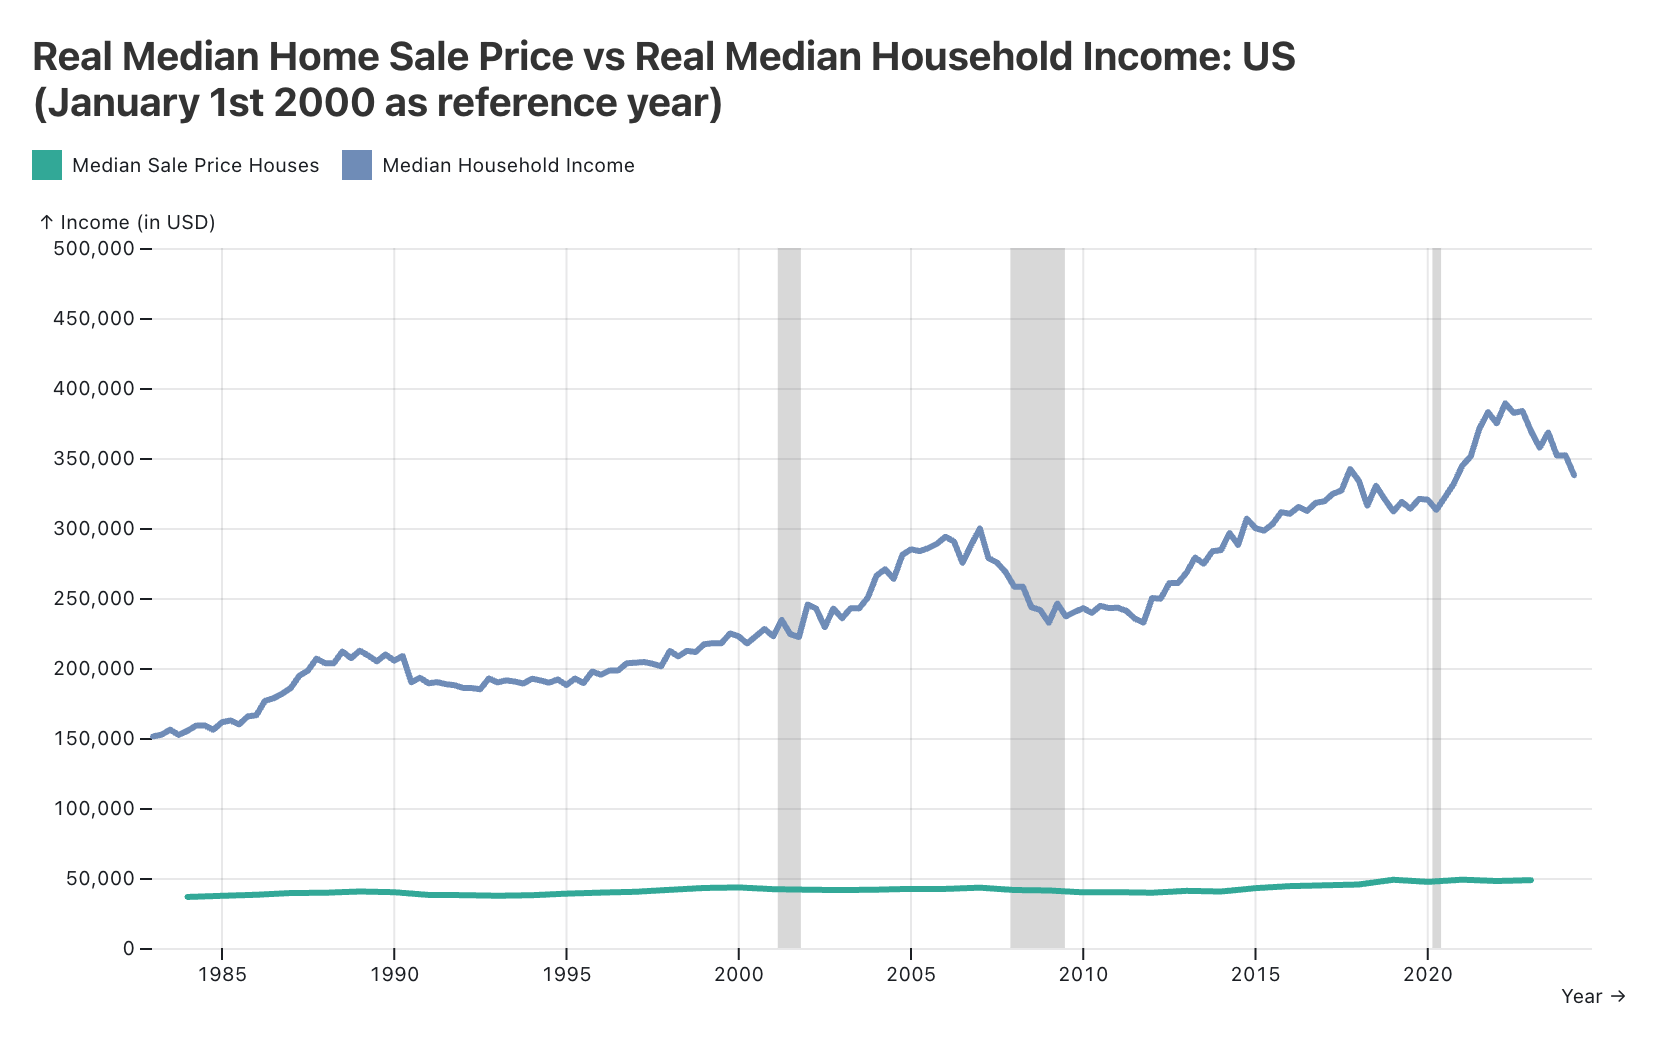
\includegraphics[width=.75\textwidth]{figs/iter4.png} 

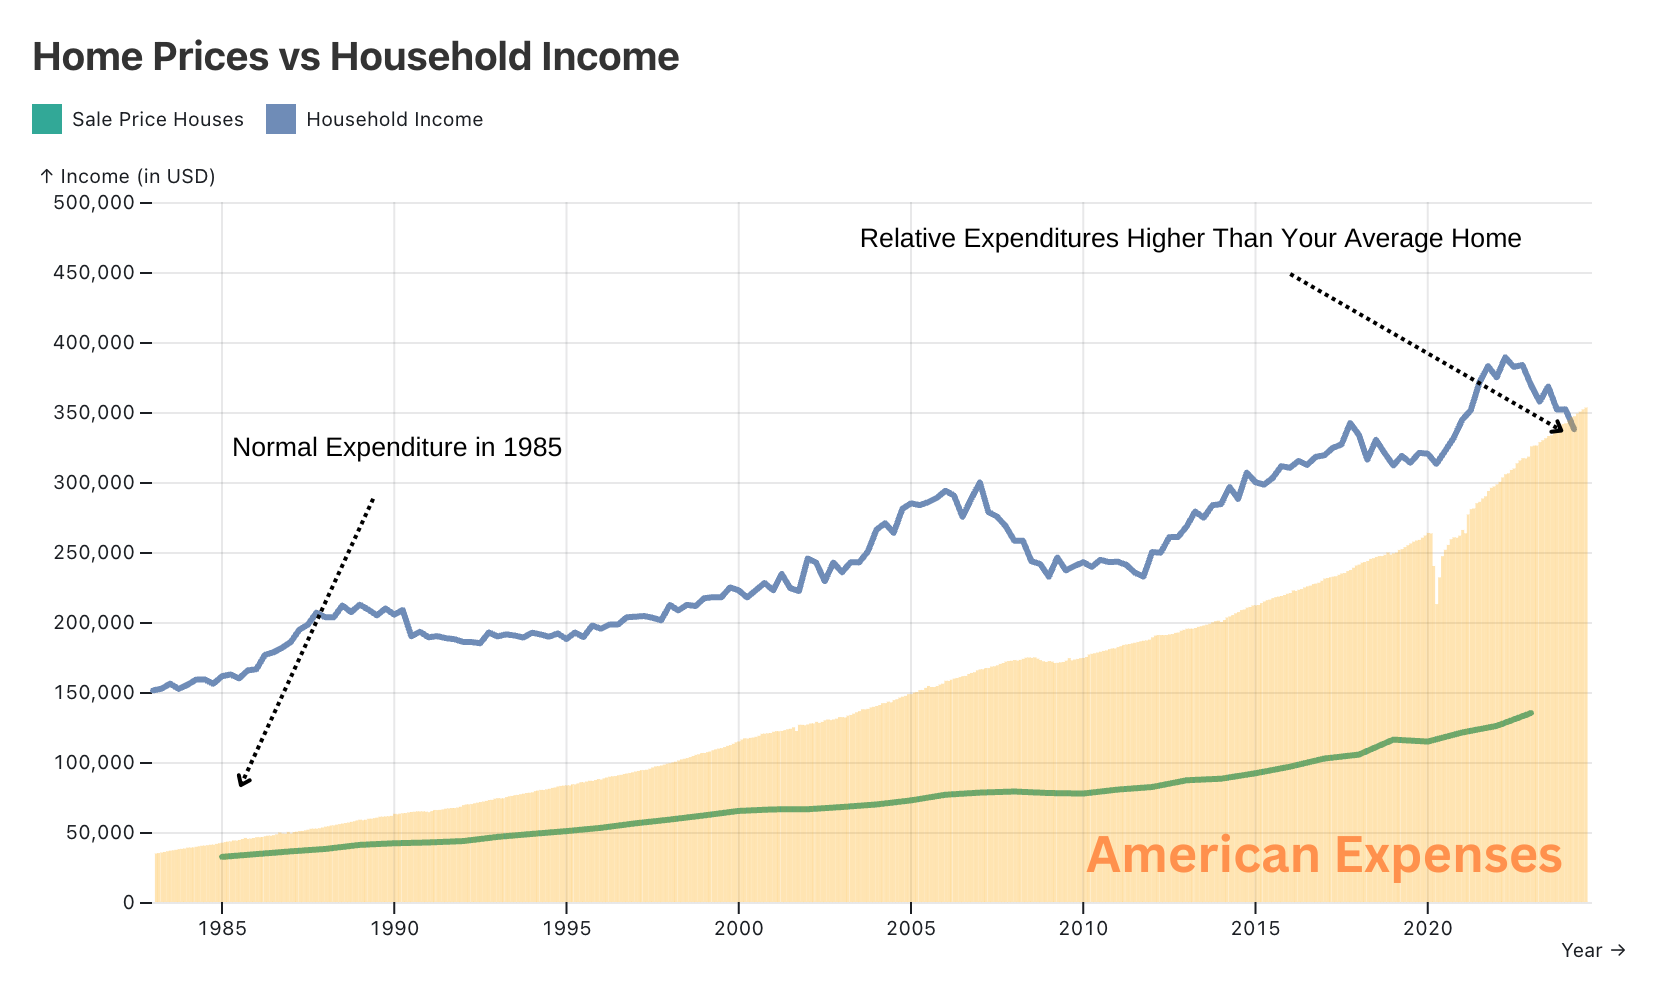
\includegraphics[width=.75\textwidth]{figs/missleading.png}

\newpage

\section{Report}
\label{sec:sec2}

\subsection{Topic Selection}
\label{subsec:topicSelection}

\subsubsection{Topic Ideation}

For the Misleading visualization I had a few ideas:

\begin{itemize}
  \item Immigration and Crime Correlations: 
  Showing an extrapolated correlation between immigration and crime rates 
  could be made misleading by selecting data points that support a biased narrative.
  For example, not filtering by region, and actively sampling from regions with high crime rates.

  \item Ethnically Biased Drug Usage: 
  Using the "US Drug overdose death rates, by drug type, sex, age, race, and Hispanic origin" 
  \cite{drugOverdoseDeathRates} dataset, we could use missleading bar charts to exaggerate the 
  correlation between hispanic heritage and drug consumption. Additionally, by 
  filtering out specific drugs we could make it especially misleading.

  \item Presidential Employment Claims:
  As much as I do not like Trump, which you'll see in the extra credit,
  the high employment rates during his presidency are largely do to the Covid-19 pandemic.
  We could use a line chart to show the employment rates over time, in contrast/comparison to Biden, 
  and by not clarifying the context of the data, we could make it seem like Trump 
  was solely responsible for the high employment rates.

  \item Immigration Crisis and Democratic Party Correlation:
  We could use a line graph to show the number of border crossings over time, and, by comparing
  Biden's and Trump's presidency, we could make it seem like the Democratic party is solely 
  responsible for the immigration crisis. This could be further exaggerated by not showing the
  Covid-19 pandemic context, and/or picking legal border crossings to be also part of the data using
  the "Border Crossing Entry Data" \cite{borderCrossingEntryData} dataset. 
  
  \item The Cost of Living vs Inflation: 
  The relation between the American people's expenditures, home prices, income, and inflation rates
  are great for generating accurate and misleading content alike. For example, one could
  greatly overvalue the spending power of the American people by not accounting for inflation rates.
  Also, by sampling subsets of the population, we could make homes seem less or more affordable than they are.
\end{itemize}

\subsubsection{Topic Selection and Question}

I decided to go with the "The Cost of Living vs Inflation" topic.

The reason why is because cost of living and income statistics lend themselves to 
both areas of the spectrum of honesty. We can sample and transform numbers 
in multiple ways, incorrecly scale items, and/or dramatize the effects of 
specific economic factors to create missleading narratives 
on the issues americans care most about. This topic also facilities my secondary goal
for this assignment: Showing how changes in data selection and visualization techniques
affect the perception of the viewer.

The question to answer is: 
\textit{Has the increase in home prices made it harder for the average American to own a home?}

I believe that this question will be perfect for evaluating both ends of the spectrum.

We will first try to generate the correct visualization of the data, answering the question
in the most clear and attentive way possible. Then, I aim to generate a visualization 
that creates confusion through various mediums. For example, the missleading visualization 
downplays, exaggerates, or eliminates important considerations like inflation,
and/or misrepresents the increase in home prices through incorrect sampling.

\subsection{Data}
\subsubsection{Required Data}
We will focus on the analysis of yearly data.

The goal was to aquire data regarding:
\begin{itemize}
  \item Home Prices: Real Home Prices, Non-Inflation Adjusted Home Prices, Home Price
  Index data, Rental Prices, Mortgage Prices, or Mortgage Rates.
  \item Income: Real Income, Non-Inflation Adjusted Income, Income Index data, or 
  household earnings.
  \item Miscelaneous: American spending habits and/or miscelaneous expenditures.
\end{itemize}

\subsubsection{Data Gathering}

All data was obtained from the Federal Reserve Economic Data (FRED) database. 
Please see \autoref{sec:apendix} for a summary of the data.

\subsection{Earnest Visualization: Iterative Improvement}
\subsubsection{Understanding The Data}

For the earnest visualization, I want to accurately show whether or not it has become
more difficult for the average american to own a home. 

We have all the necessary data to answer this question, specifically, for plotting the
real wages of the average american against the real home prices.

To eliminate all possible bias, we will use the Real Median Household Income 
and the Real Residential Property Prices datasets. By using the median of household income,
we can avoid the bias of outliers, more accurately showing the average american, 
and, by using the real prices, we can avoid the bias of inflation. 

Let's visualize the bias I am talking about:

\begin{figure}[ht] 
  \centering
  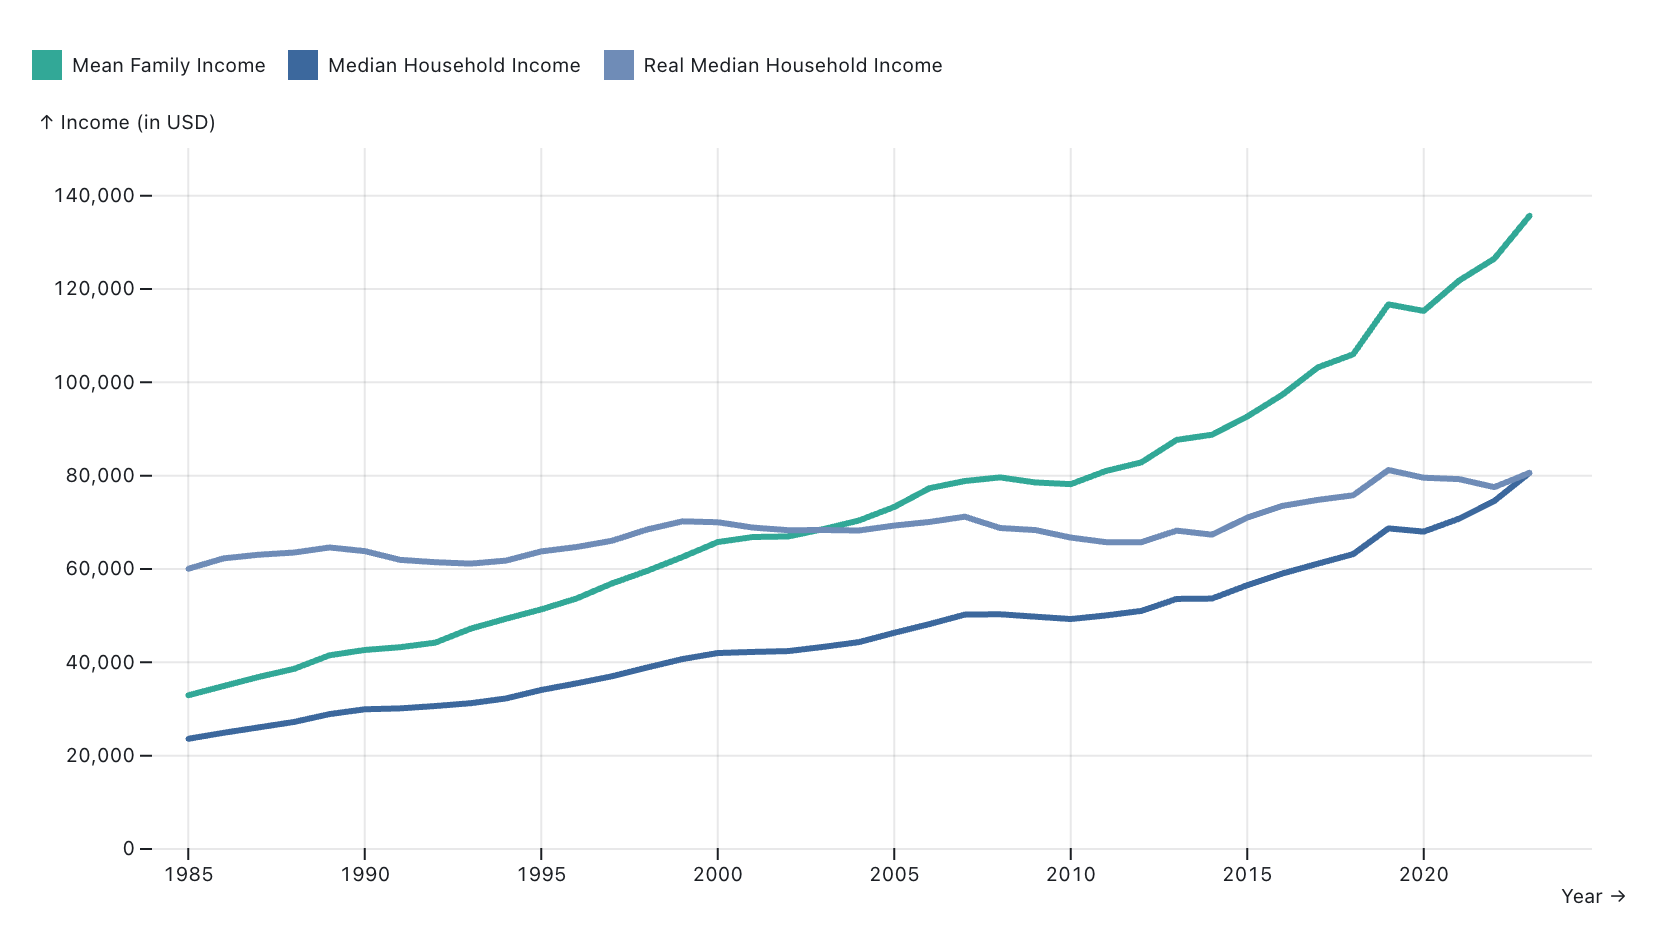
\includegraphics[width=.90\textwidth]{figs/income.png}
  \caption{
      To much of the dismay of my fellow compatriots, the real median household income has been pretty stagnant. \\
      However, do realize that we can misrepresent the income of americans by forgetting this fact.
  }
  \label{fig:income}
\end{figure}

\subsubsection{Iterative Improvement}

For the first iteration, I plotted the Real Median Household Income against the Real Residential Property Prices.

\begin{figure}[ht] 
  \centering
  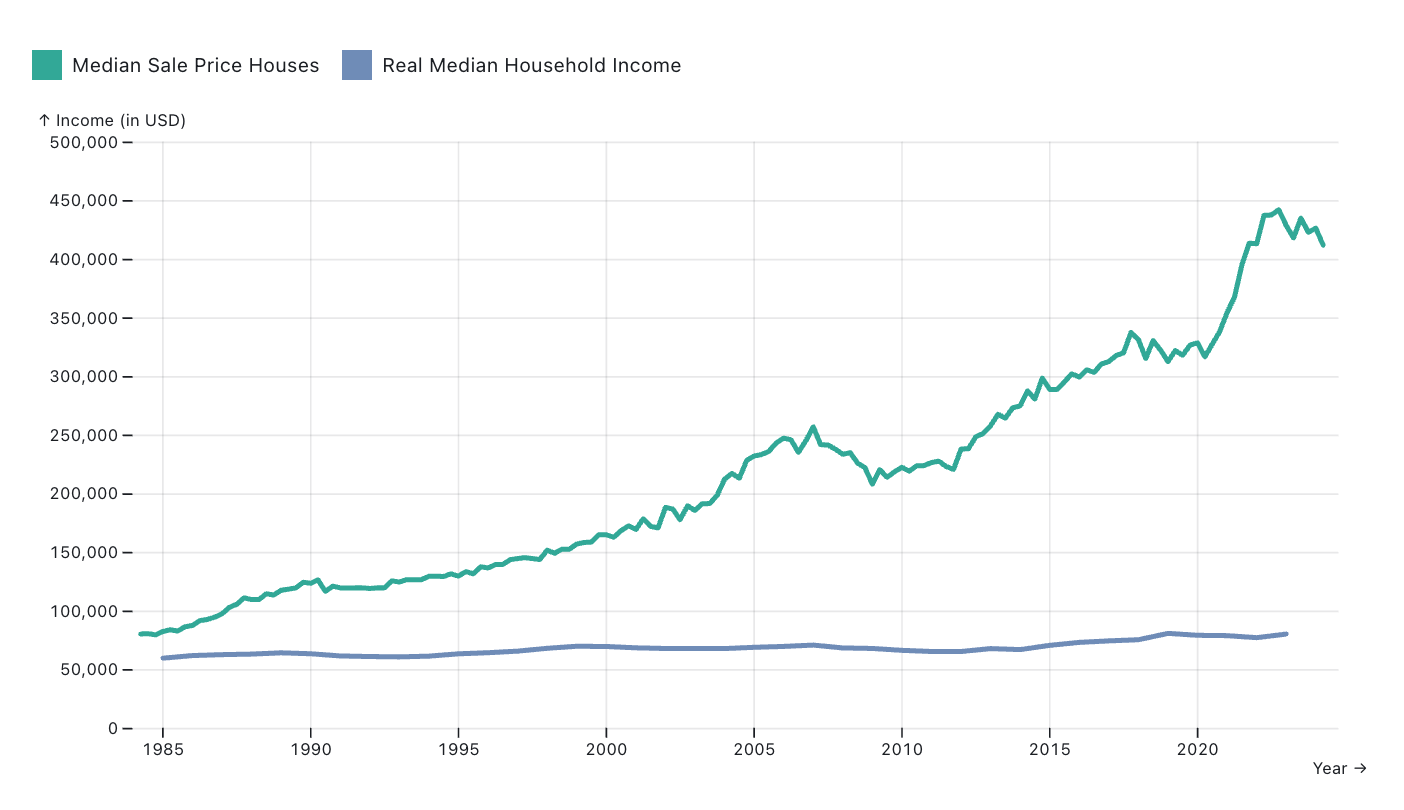
\includegraphics[width=.90\textwidth]{figs/iter1.png}
  \caption{
      Real Median Household Income vs Residential Property Prices
  }
  \label{fig:iter1}
\end{figure}

\autoref{fig:iter1} does not take inflation into account, so, for our earnest visualization we have two options:

\begin{itemize}
  \item Adjust the Real Median Household Income for inflation.
  \item Utilize Median Household Income without adjusting for inflation, which would represent the price paid for homes in the year of purchase.
\end{itemize}

Both options are totally fine, but I will go with the first option, since we want to make an appeal to modern individuals. 

\begin{figure}[ht] 
  \centering
  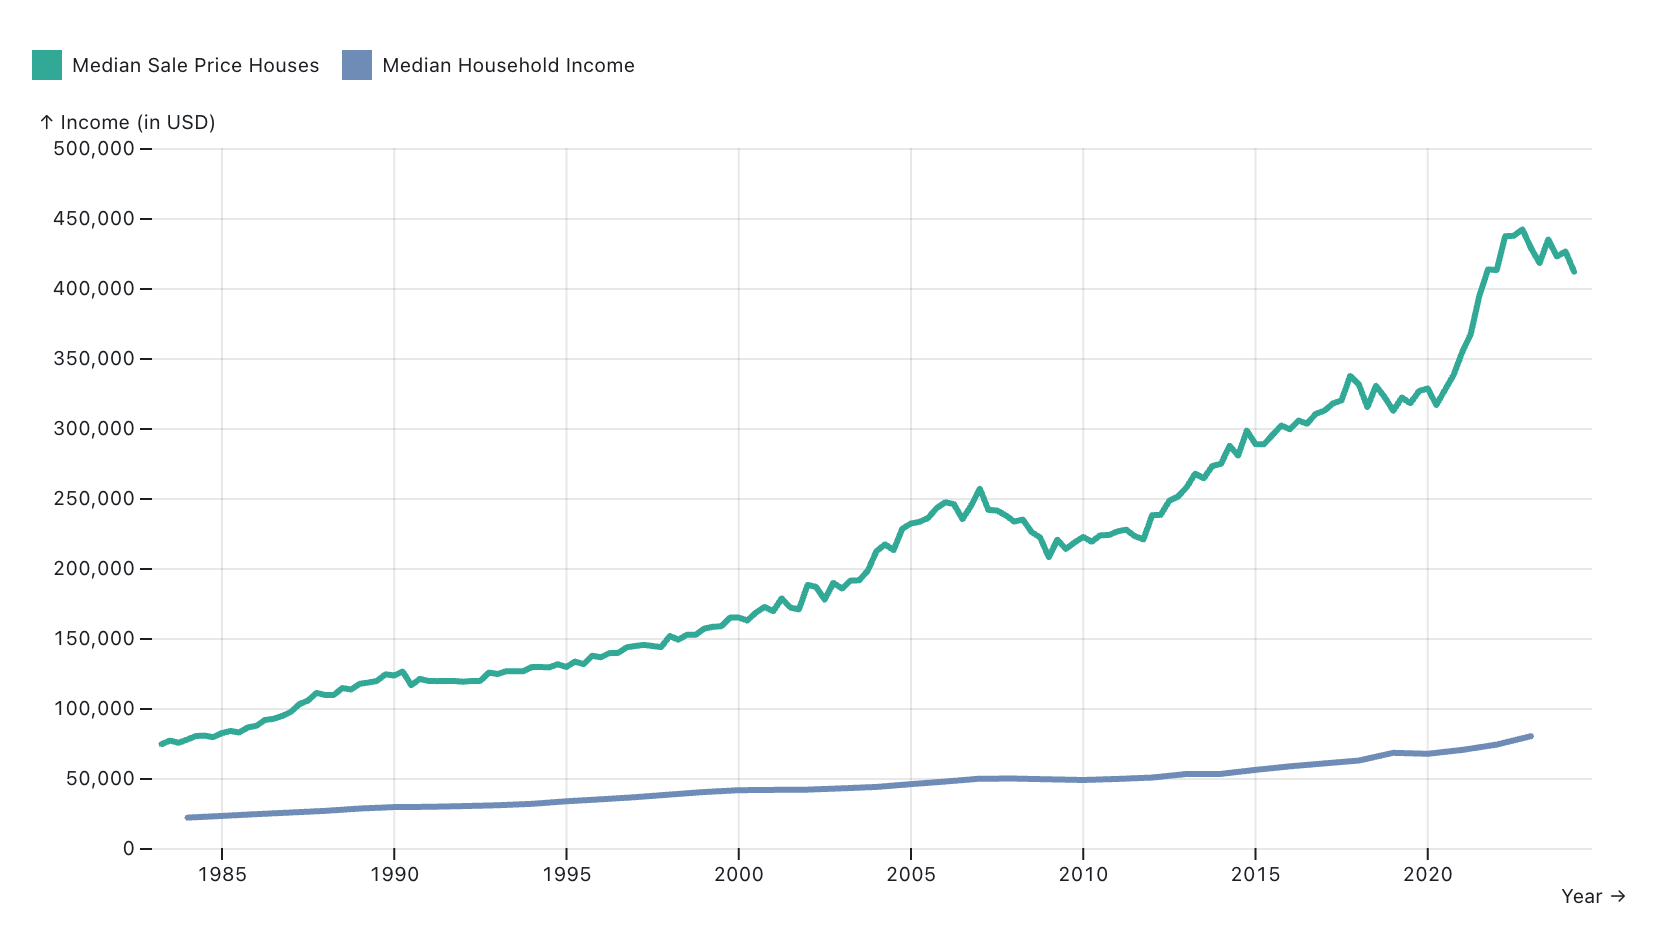
\includegraphics[width=.75\textwidth]{figs/iter2.png}
  \caption{
      Median Household Income vs Residential Property Prices (No Inflation Adjustment)
  }
  \label{fig:iter2}
\end{figure}

In \autoref{fig:iter2} we can see both values without inflation adjustments.

In \autoref{fig:iter3}, we can see the values with inflation adjustments. 
This was done by taking the Consumer Price Index for All Urban Consumers dataset 
and dividing dollar values for both nominal datasets by it, using the year 2000 as the base year.

\begin{figure}[ht] 
  \centering
  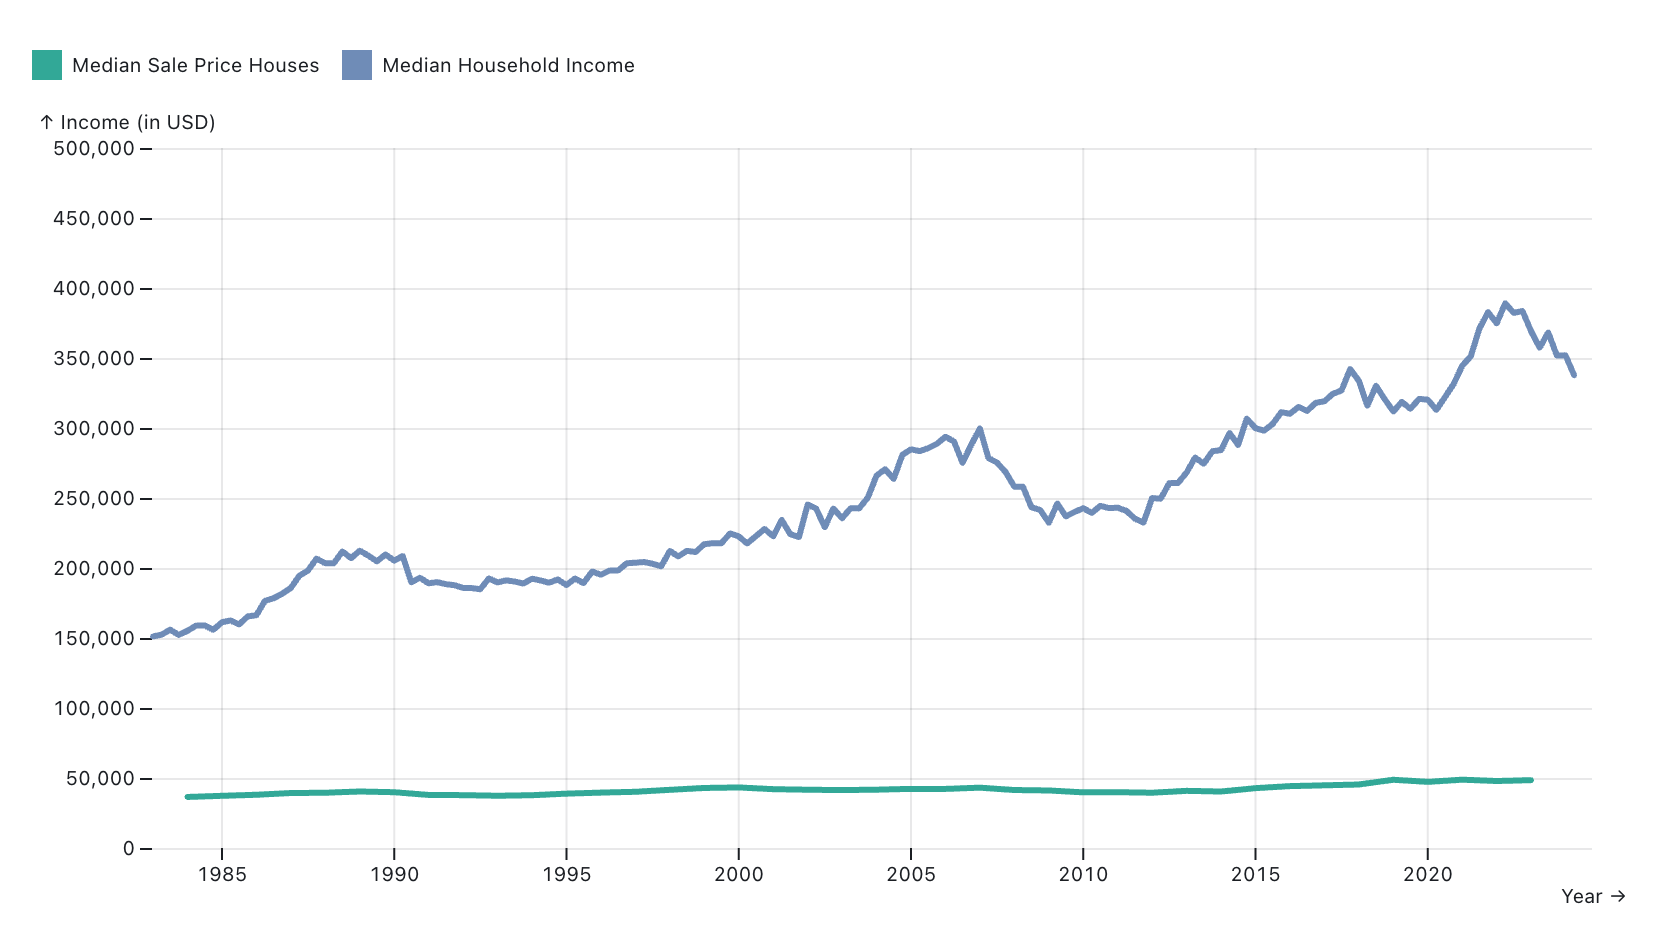
\includegraphics[width=.75\textwidth]{figs/iter3.png}
  \caption{
      Median Household Income vs Residential Property Prices (No Inflation Adjustment)
  }
  \label{fig:iter3}
\end{figure}

Finally, for the earnest visualization, we will add two goodies to improve the visuals:
\begin{itemize}
  \item A clear title that is not optionated.
  \item A highlight of recession years to further indicate home price fluctuations.
\end{itemize}

\begin{figure}[ht] 
  \centering
  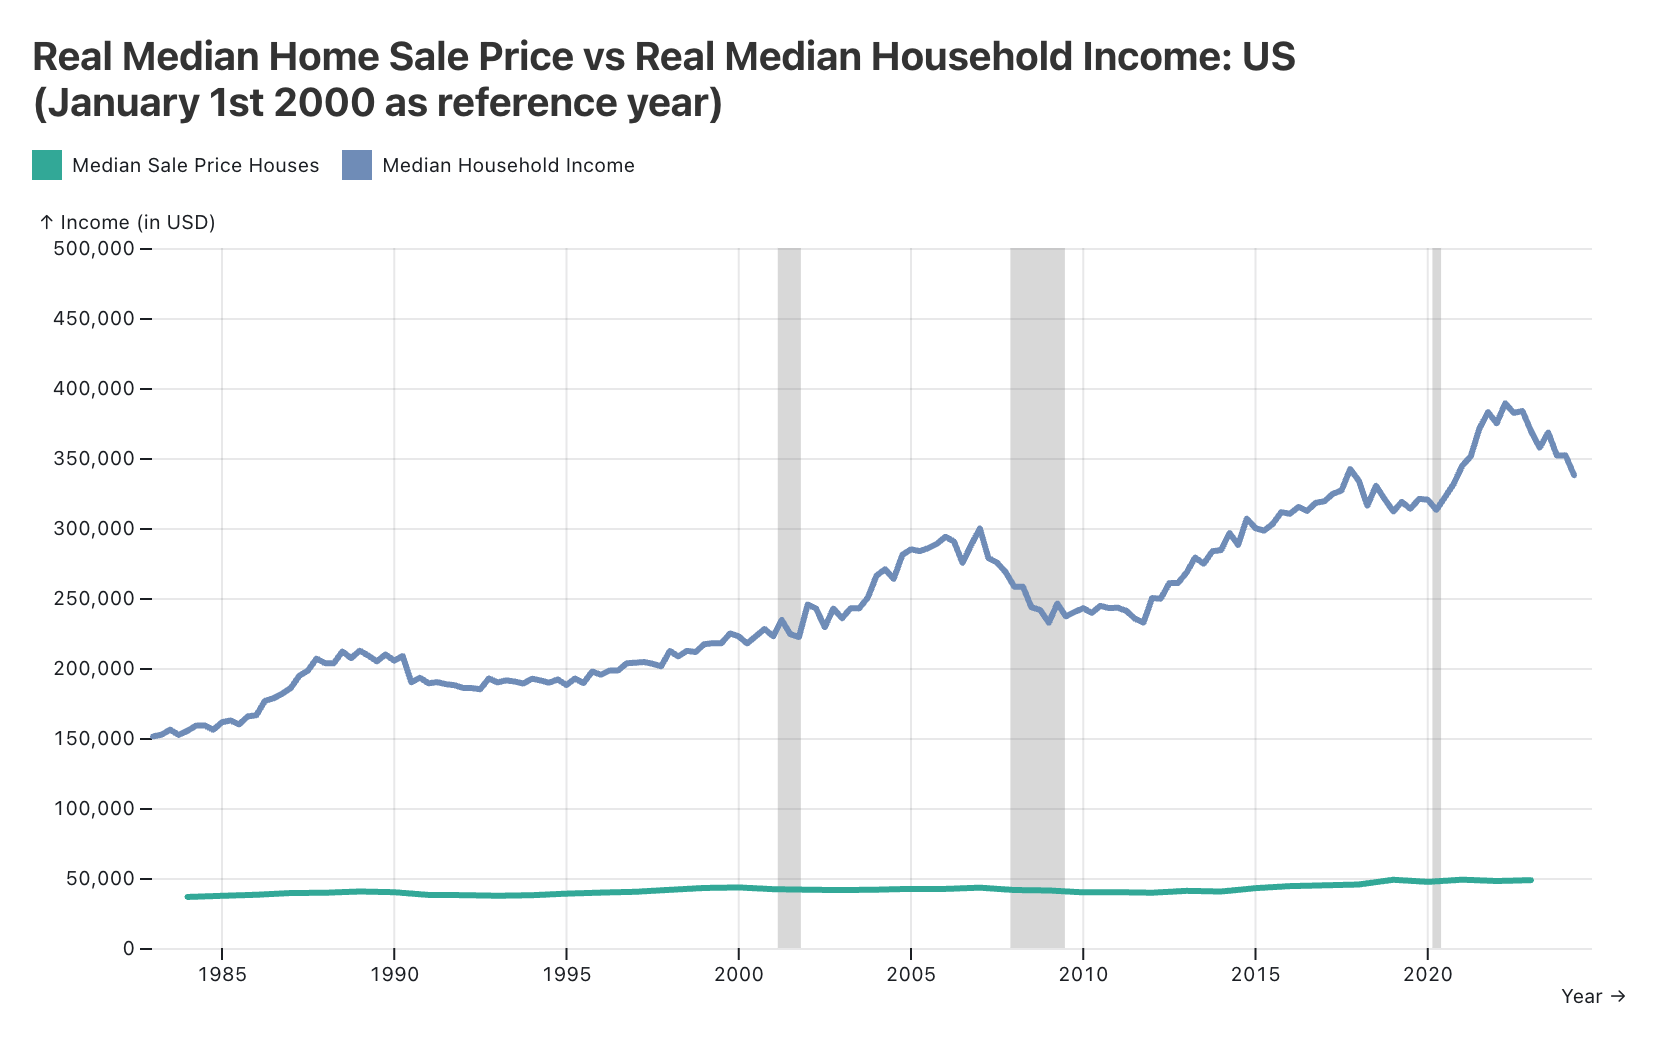
\includegraphics[width=.75\textwidth]{figs/iter4.png}
  \caption{
      Final Visualization. Beatufiul, prestine, and honest.
  }
  \label{fig:iter4}
\end{figure}

Hopefully, I have convinced you that there is a disconnect between home prices and income. 
Please note that the upmost financial care was put into the numbers. The problem is real. 
Let's see how we can maliciously flip the script.

\newpage

\subsection{Missleading Visualization}
\subsubsection{Iterative Deceit}

For the missleading visualization, we will reuse the normalized home price dataset.

However, we will use the Nominal Mean Family Income dataset, for maximum deceit.

Additionally, we will include a non-normalized figure of personal expenditures, to further confuse the viewer.

Hopefully, we can make the viewer believe that the average american is spending more than they are earning,
and that that is the reason why they cannot afford a home. By the way, we are intentionally leaving out the rule here,
since this is an index, and plotting it correctly would give things away.

\begin{figure}[ht] 
  \centering
  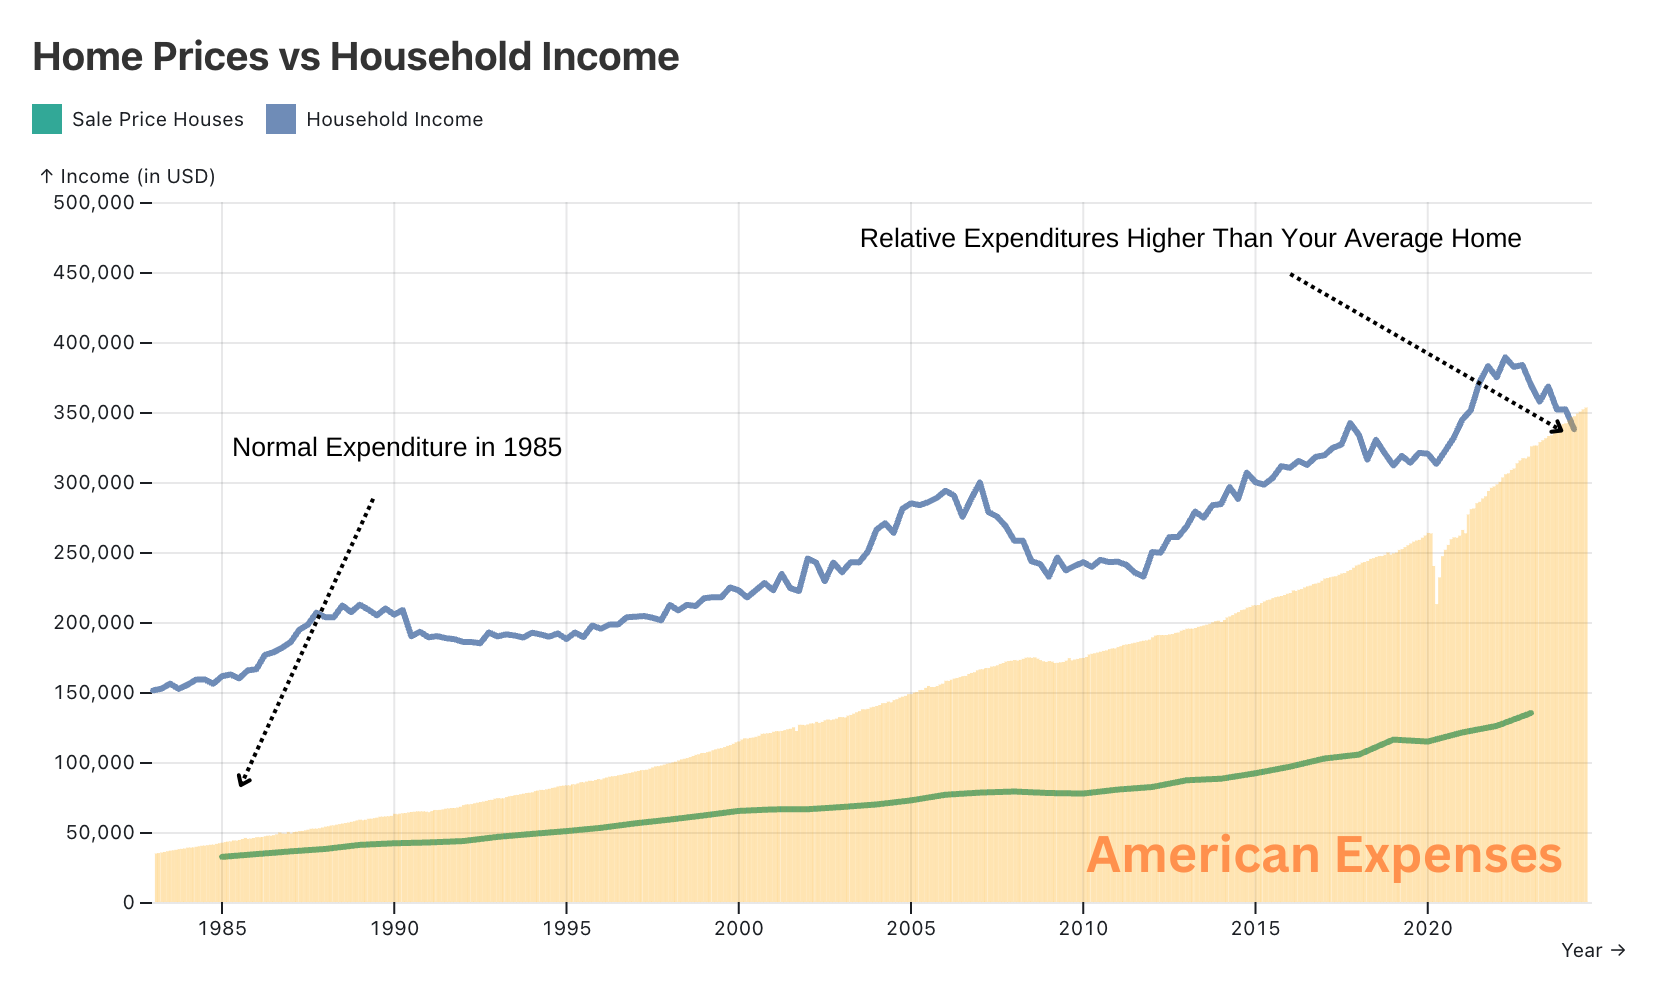
\includegraphics[width=.75\textwidth]{figs/missleading.png}
  \caption{
      Missleading Visualization. The average american is spending more than they are earning.
  }
  \label{fig:missleading}
\end{figure}
\subsubsection{Effectiveness}

I think that this visualization is perfect for confirming an inherent bias in the viewer.

My goal was to show the viewer that the average american has been earning more money, and that, 
relative to the price of houses, they are more or less the same as they were in the past.

However, by including the personal expenditures, 
I have made it seem like the average american is spending more than they are earning.
Wrongly allowing them to conclude that the problem is with the mentality of young american people, and not with policy.

Of course, these is all bologna. The average american is earning less, and the price of homes has skyrocketed.

\newpage
\section{Apendix}
\label{sec:apendix}


\textbf{Income, Earnings, and Revenue}
\begin{itemize} 
  \item \textbf{Mean Family Income} 
  \begin{itemize} 
    \item \textbf{Series ID}: \texttt{MAFAINUSA646N} 
    \item \textbf{Units}: Current dollars 
  \end{itemize}

  \item \textbf{Nominal Median Household Income} 
  \begin{itemize} 
    \item \textbf{Series ID}: \texttt{MEHOINUSA646N} 
    \item \textbf{Units}: Current dollars 
  \end{itemize}

  \item \textbf{Real Median Household Income}
  \begin{itemize}
      \item \textbf{Series ID}: \texttt{MEHOINUSA672N}
      \item \textbf{Units}: Constant dollars (adjusted for inflation)
  \end{itemize}

  \item \textbf{Income Before Taxes (Wages and Salaries) by Age (from Age 25 to 34)}
  \begin{itemize}
      \item \textbf{Series ID}: \texttt{CXU900000LB0403M}
      \item \textbf{Units}: Current Dollars
  \end{itemize}
\end{itemize}

\textbf{Housing Related}
\begin{itemize} 
  \item \textbf{Average Sales Price of Houses Sold}
  \begin{itemize}
      \item \textbf{Series ID}: \texttt{ASPUS}
      \item \textbf{Units}: Current Dollars
  \end{itemize}

  \item \textbf{Median Sales Price of Houses Sold}
  \begin{itemize}
      \item \textbf{Series ID}: \texttt{MSPUS}
      \item \textbf{Units}: Current Dollars
  \end{itemize}
  
  \item \textbf{Housing Affordability Index}
  \begin{itemize}
      \item \textbf{Series ID}: \texttt{FIXHAI}
      \item \textbf{Units}: Index
  \end{itemize}
\end{itemize}

\textbf{Personal Consumption}
\begin{itemize}
  \item \textbf{Real Personal Consumption Expenditures}
  \begin{itemize}
      \item \textbf{Series ID}: \texttt{PCEC96}
      \item \textbf{Units}: Billions of Chained 2017 Dollars
  \end{itemize}

  \item \textbf{Personal Consumption Expenditures}
  \begin{itemize}
      \item \textbf{Series ID}: \texttt{PCE}
      \item \textbf{Units}: Billions of Current Dollars
  \end{itemize}

  \item \textbf{Personal Consumption Expenditures Excluding Food and Energy}
  \begin{itemize}
      \item \textbf{Series ID}: \texttt{DPCCRC1M027SBEA}
      \item \textbf{Units}: Billions of Current Dollars
  \end{itemize}
\end{itemize}

\textbf{Inflation}
\begin{itemize}
  \item \textbf{Consumer Price Index for All Urban Consumers: All Items in U.S. City Average}
  \begin{itemize}
      \item \textbf{Series ID}: \texttt{CPIAUCSL}
      \item \textbf{Units}: Index 1982-1984=100
  \end{itemize}
\end{itemize}    

\newpage
\begin{refcontext}[sorting=nyt]
\printbibliography
\end{refcontext}

\end{document}

